\documentclass[10pt]{article}
\usepackage[margin=0.8in]{geometry}
\usepackage{booktabs,graphicx,float,xcolor,enumitem,microtype,multirow,caption}
\usepackage[hidelinks]{hyperref}
\usepackage{amsmath}
\setlist{nosep,leftmargin=*}
\captionsetup{font=small,labelfont=bf}
\newcommand{\RES}[1]{\textcolor{red}{[#1]}}
\setlength{\parskip}{3pt}\setlength{\parindent}{0pt}

\title{\vspace{-2em}Instruction Tuning and DPO on Qwen2.5-0.5B\\\large CS5326 Programming Assignment 2}
\author{Roll no. 27100172}
\date{October 2026}

\begin{document}
\maketitle
\vspace{-1.5em}

\section{Repository, Models, and Data}
\textbf{Code:} \url{https://github.com/whyeventry0103/cs5326-pa2-27100172} (private until submission).
SFT and both DPO runs are hand-written loops in \texttt{src/alignment} and \texttt{scripts/train\_\{sft,dpo\}.py}; no HF \texttt{Trainer} or TRL is used for them. \texttt{submission\_adapter.py} wraps this code and passes the public tests plus 14 additional edge-case tests (\texttt{tests/test\_alignment\_core.py}).

\textbf{Base checkpoints.} \texttt{Qwen/Qwen2.5-0.5B} (SFT, DPO); \texttt{HuggingFaceTB/SmolLM2-360M-Instruct} (LoRA-DPO).

\textbf{Data} (all subsets built by \texttt{scripts/prepare\_data.py}, seed 42: shuffle indices, keep the first $n$ rows that pass the filters).
\begin{itemize}
\item \textbf{SFT:} \texttt{HuggingFaceH4/ultrachat\_200k}, first user/assistant turn only; 30{,}000 train (\texttt{train\_sft}) and 1{,}000 validation (\texttt{test\_sft}). Filter: formatted prompt + response + EOS $\le$ 512 tokens, so the EOS is always learned and never truncated away (mean response 165 words).
\item \textbf{HH-RLHF DPO:} \texttt{Anthropic/hh-rlhf}, single-turn transcripts only (exactly one Human and one Assistant turn), identical prompt in chosen/rejected, non-identical non-empty responses, formatted prompt $\le$ 256 tokens; 15{,}000 train / 1{,}000 val (\texttt{test} split).
\item \textbf{UltraFeedback DPO:} \texttt{HuggingFaceH4/ultrafeedback\_binarized}, single-turn, strict preferences only (\texttt{score\_chosen} $>$ \texttt{score\_rejected}; ties are dropped), same prompt-length filter; 15{,}000 \texttt{train\_prefs} / 1{,}000 \texttt{test\_prefs}.
\item \textbf{Persona LoRA-DPO:} the provided 220 rows of \texttt{ramsay\_style\_preferences.json}; 200 train / 20 held-out (seeded shuffle).
\end{itemize}
Chosen responses are longer than rejected ones in 54\% (HH) and 57\% (UF) of training pairs, a mild length signal relevant to \S\ref{sec:analysis}.

\textbf{Evaluation sets} (all in \texttt{eval\_sets/}): the provided synthetic HH set (300 prompts, 10 categories $\times$ 30); AlpacaEval, 300 prompts sampled with \texttt{random.Random(42).sample} from the 805-prompt \texttt{alpaca\_eval.json} (\texttt{alpaca\_eval\_300\_seed42.json}, source indices stored); and a 40-prompt persona set I wrote (10 each: cooking, coding, general help, safety-sensitive), checked for no overlap with the persona training prompts.

\textbf{Prompt format.} One explicit ChatML template for SFT, DPO and generation (\texttt{src/alignment/prompting.py}):
\texttt{<|im\_start|>system\textbackslash nYou are a helpful assistant.<|im\_end|>\textbackslash n<|im\_start|>user\textbackslash n\{x\}<|im\_end|>\textbackslash n<|im\_start|>assistant\textbackslash n}, followed by the response and the tokenizer EOS (\texttt{<|endoftext|>}). The prompt and response are tokenized separately and concatenated; EOS is appended before right-truncation to \texttt{max\_length}; prompt and pad positions get label $-100$. Masks are derived from positions, not token ids, because Qwen's pad and EOS ids coincide. SmolLM2 uses its own chat template through TRL.

\section{Experimental Configuration}
\begin{table}[H]\centering\small
\caption{Values actually used for the submitted checkpoints. All seeds 42; one epoch unless noted.}
\label{tab:config}
\resizebox{\linewidth}{!}{%
\begin{tabular}{lllll}
\toprule
 & \textbf{SFT} & \textbf{HH-RLHF DPO} & \textbf{UltraFeedback DPO} & \textbf{LoRA-DPO (persona)} \\
\midrule
Init / reference & Qwen2.5-0.5B & SFT \texttt{best} / frozen SFT \texttt{best} & SFT \texttt{best} / frozen SFT \texttt{best} & SmolLM2-360M-Instruct / adapter-disabled base \\
Trainable & full (494M) & full & full & LoRA r=16, $\alpha$=32, drop 0.05, q,k,v,o,gate,up,down \RES{params} \\
Objective & response-token NLL (token mean) & DPO, $\beta=0.1$ & DPO, $\beta=0.1$ & DPO $\beta=0.1$ + 1.0$\times$ chosen NLL (TRL \texttt{["sigmoid","sft"]}) \\
Optimizer & AdamW (0.9, 0.999), wd 0.1 & AdamW, wd 0 & AdamW, wd 0 & AdamW (TRL default), wd 0 \\
Peak LR / schedule & $2\!\times\!10^{-5}$, 3\% warmup (28 steps), cosine & $10^{-6}$ constant & $10^{-6}$ constant & $2\!\times\!10^{-4}$, 10\% warmup, cosine \\
Grad clip & 1.0 & 1.0 & 1.0 & 1.0 \\
Batch (dev $\times$ accum = eff.) & 2 $\times$ 16 = 32 & 1 pair $\times$ 32 = 32 & 1 pair $\times$ 32 = 32 & 4 $\times$ 2 = 8 \\
Steps / epochs & 937 / 1 & \RES{468} / 1 & \RES{468} / 1 & 75 / 3 \\
Precision & fp16 autocast, fp32 master weights, GradScaler & same; fp32 reference under same autocast & same & bf16 \\
Max length (prompt) & 512 & 512 (256) & 512 (256) & 512 \\
Selected ckpt & best val loss (step 937) & best val reward acc. (step \RES{}) & best val reward acc. (step \RES{}) & end of training \\
\bottomrule
\end{tabular}}
\end{table}
\textbf{Generation (all Qwen models identical):} greedy, \texttt{max\_new\_tokens}=512, \texttt{repetition\_penalty}=1.2, no n-gram blocking, stop on \texttt{<|endoftext|>} or \texttt{<|im\_end|>}, bf16, same ChatML template. Persona (both SmolLM2 models): greedy, 256 new tokens, no penalty, SmolLM2 chat template. Temperature and top-$p$ are unused under greedy decoding.

\section{Parameter Choices and Deviations}
\textbf{Resource/environment-driven.}
\begin{itemize}
\item \textit{Hardware:} runs used a shared 2$\times$RTX 6000 Ada server instead of Kaggle T4$\times$2, with only $\sim$14\,GB free per GPU. I kept the T4 recipe (fp16 autocast + GradScaler, the same batch sizes) so the numbers remain comparable to the guide configuration.
\item \textit{DPO placement:} the guide places the policy on \texttt{cuda:0} and the reference on \texttt{cuda:1}. On this server, direct GPU-to-GPU copies silently returned zeros, which zeroed the reference log-probs (step-0 reward margin $-4.47$ instead of $0$). I fixed this by staging cross-device copies through host memory, added a guard that aborts if step-0 rewards are non-zero, and ran each DPO job with policy and reference on the same GPU (12.5\,GB peak with gradient checkpointing). The reference is kept in fp32, not fp16, so step-0 rewards are exactly zero (manual \S10.5).
\item \textit{Judge location:} the Kaggle model proxy was used only for judging (\S\ref{sec:results}); everything else ran on the server.
\end{itemize}
\textbf{Performance-driven.}
\begin{itemize}
\item \textit{Decoding:} greedy decoding from the SFT model looped (``a meat thermometer'' $\times$50). In a 4-prompt sanity check, \texttt{repetition\_penalty}=1.1 still looped and 1.2 did not, so 1.2 is used for every Qwen model in every comparison.
\item \textit{LoRA-DPO:} the guide-like setting (lr $5\!\times\!10^{-5}$, plain DPO) reached 100\% held-out preference accuracy, yet generations were barely in persona. Raising the LR made plain DPO collapse into repetition loops. Adding an NLL term on the chosen responses (RPO-style) fixed fluency. Table~\ref{tab:sweep} summarizes the sweep.
\end{itemize}
\begin{table}[H]\centering\small
\caption{LoRA-DPO sweep (3 epochs, r=16). Pref.\ acc./margin: TRL metrics on the 20 held-out pairs. Style proxies on the 40 persona prompts: share of responses with a signature insult from the training data (``you donkey/donut/\ldots''), exclamation marks per response, mean words, share hitting the 256-token cap (repetition loops), and insult share on the 10 safety-sensitive prompts. \textbf{Bold}: submitted.}
\label{tab:sweep}
\begin{tabular}{lccccccc}
\toprule
Config & Pref.\ acc. & Margin & Insult & ! / resp & Words & Hit cap & Insult (safety) \\
\midrule
SmolLM2-360M-Instruct (no LoRA) & -- & -- & 0\% & 0.1 & 112 & 40\% & 0\% \\
lr=5e-5, $\beta$=0.1, plain DPO & 1.00 & 1.95 & 0\% & 2.0 & 141 & 50\% & 0\% \\
lr=1e-4, $\beta$=0.1, plain DPO & 1.00 & 5.03 & 0\% & 15.7 & 167 & 90\% & 0\% \\
lr=1e-4, $\beta$=0.5, plain DPO & 1.00 & 9.94 & 0\% & 2.2 & 150 & 62\% & 0\% \\
lr=2e-4, $\beta$=0.1, plain DPO & 1.00 & 9.04 & 0\% & 18.4 & 141 & 100\% & 0\% \\
lr=5e-5, $\beta$=0.1, +NLL & 1.00 & 1.87 & 0\% & 1.6 & 128 & 52\% & 0\% \\
lr=1e-4, $\beta$=0.1, +NLL & 1.00 & 3.32 & 2\% & 2.5 & 44 & 8\% & 10\% \\
\textbf{lr=2e-4, $\beta$=0.1, +NLL} & 1.00 & 4.78 & 78\% & 2.9 & 35 & 2\% & 80\% \\
\bottomrule
\end{tabular}
\end{table}


\section{Training Behavior}
\begin{figure}[H]\centering
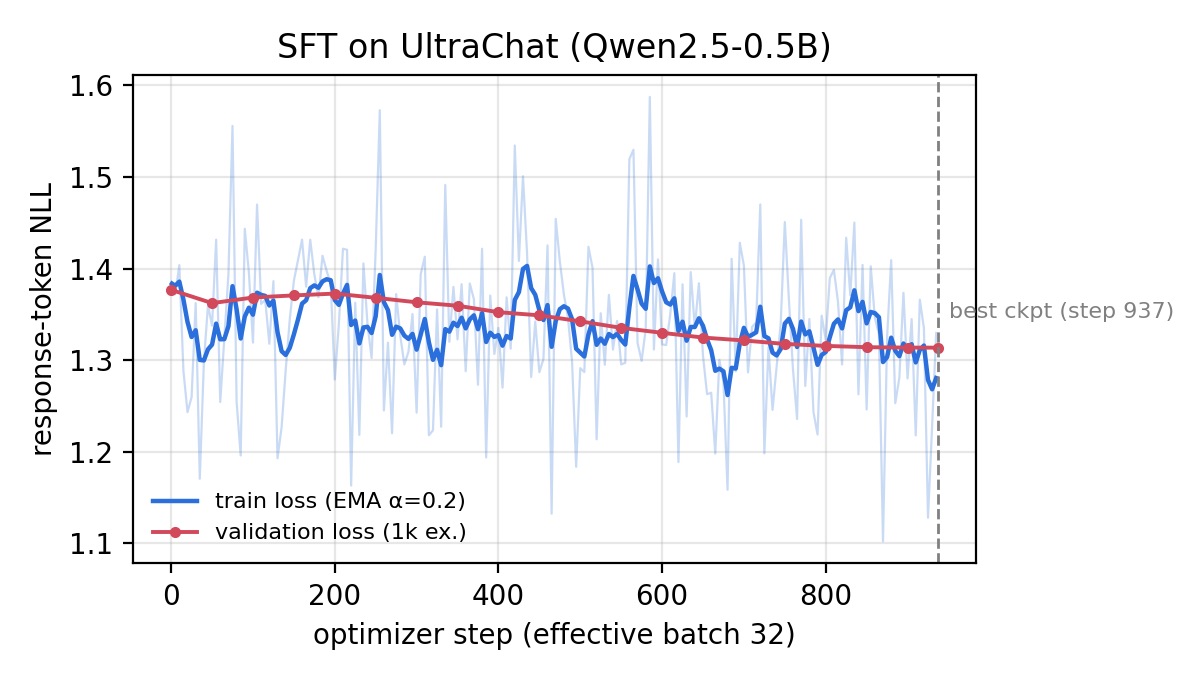
\includegraphics[width=0.49\linewidth]{figures/sft_loss.png}\hfill
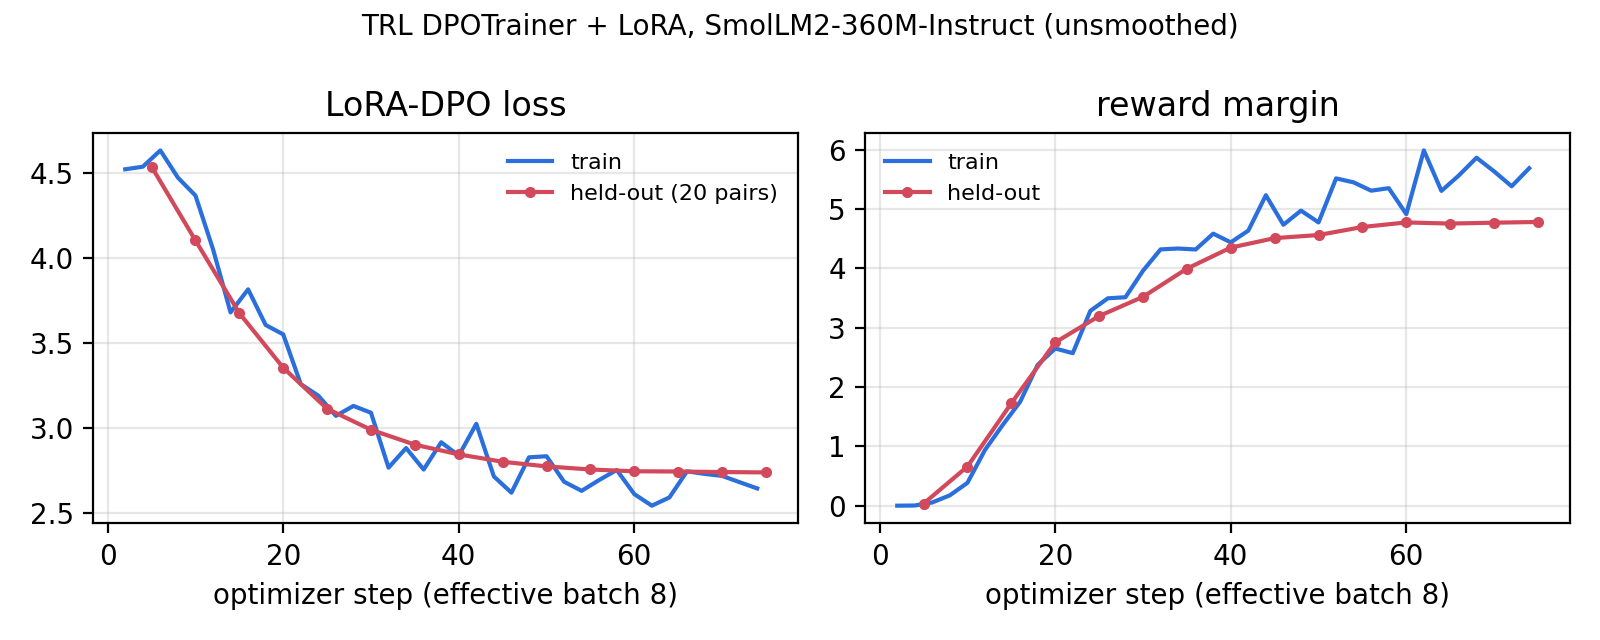
\includegraphics[width=0.49\linewidth]{figures/lora_dpo.png}
\caption{Left: SFT train loss (raw and EMA) and validation loss. Right: LoRA-DPO loss and reward margin (TRL logs).}
\label{fig:sft}
\end{figure}
\begin{figure}[H]\centering
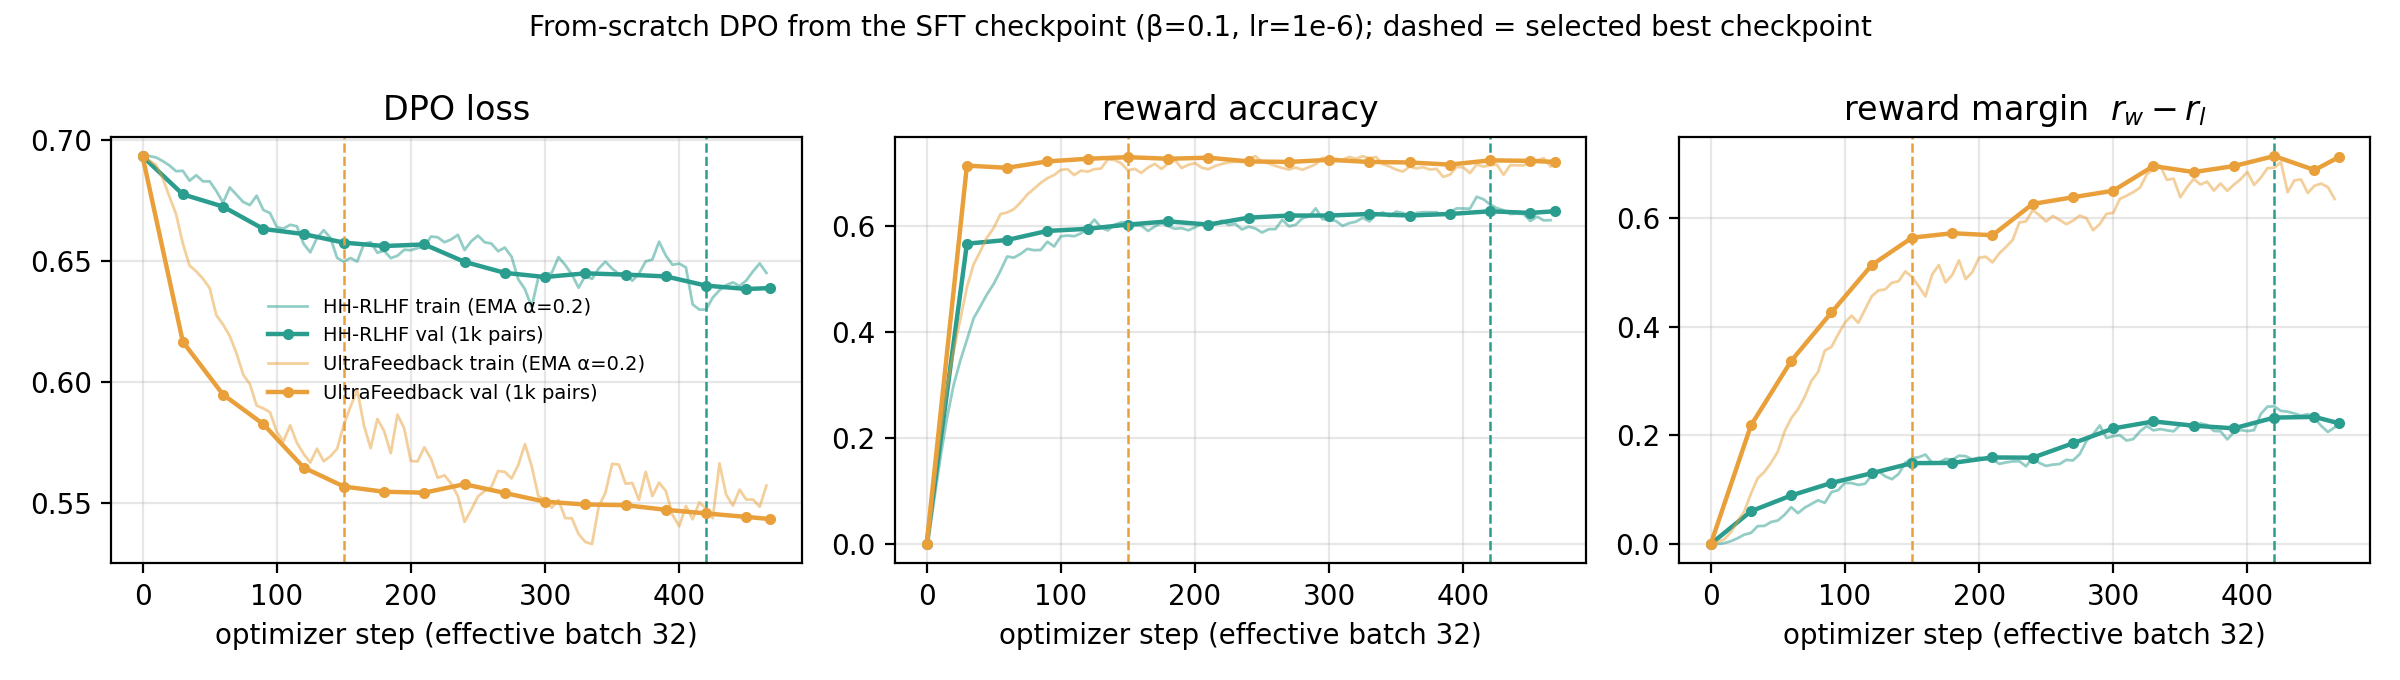
\includegraphics[width=\linewidth]{figures/dpo_curves.png}
\caption{From-scratch DPO. Train curves are EMA-smoothed per-step means over 32 pairs; validation points are on the full 1k pairs; dashed lines mark the selected checkpoints.}
\label{fig:dpo}
\end{figure}
\textbf{SFT} (38 min). Validation NLL fell from 1.377 to 1.362 in the first 50 steps, \emph{rose} to 1.373 around the peak learning rate (steps 100--200), then decreased monotonically as the cosine schedule decayed, ending at 1.314. Best and final coincide (step 937), so there is no sign of overfitting in one epoch. Per-batch training loss is noisy (1.1--1.6 for 32 examples; median pre-clip gradient norm 4.0), so the EMA is shown. The early bump suggests $2\times10^{-5}$ is near the upper end for full fine-tuning of this model: the base model already models UltraChat-style text well (initial NLL 1.38).

\textbf{HH-RLHF DPO} (61 min). At step 0 the loss is exactly $\ln 2$ with all rewards 0 (reward accuracy 0, as \S10.5 predicts). Validation reward accuracy rose quickly to 0.566 (step 30), then slowly to 0.627 (step 420, selected); the margin grew from 0.06 to 0.23 and the loss fell to 0.640. Both implicit rewards became \emph{negative} (chosen $-0.45$, rejected $-0.68$ at the selected step): DPO widened the gap mainly by lowering the rejected likelihood while the chosen log-probability also drifted down (policy chosen log-prob $-185.6 \to -191.0$). HH pairs are noisy (the chosen reply is often only marginally better), which matches the modest ceiling.

\textbf{UltraFeedback DPO} (72 min). Reward accuracy jumped to 0.713 by step 30 and then plateaued at 0.72--0.73 (best 0.729 at step 150, selected by the manual's rule), while the margin kept growing from 0.56 to 0.71 and the loss kept falling (0.557 $\to$ 0.543). Accuracy differences after step 30 are within one standard error ($\approx$1.4 pp on 1k pairs), so ``best'' is essentially an early-stopping choice. Here too the gain comes from pushing rejected responses down (rejected reward $-0.54$ vs chosen $+0.02$ at step 150). In both runs the pre-clip gradient norm (median 42--57) is far above the clip of 1.0, so every update is clipped; with AdamW this mostly rescales the moment estimates. The fp16 GradScaler skipped one or two initial steps while calibrating.

\textbf{LoRA-DPO.} With the added chosen-NLL term the logged loss (DPO + NLL) falls from 4.5 to 2.7. Held-out preference accuracy is 1.0 from step 10 and the margin saturates near 4.8, so these 20 pairs cannot separate configurations; Table~\ref{tab:sweep} uses generation-level diagnostics instead.

\section{DPO-versus-SFT Results}\label{sec:results}
\RES{results table + text}

\section{Interpretation and Error Analysis}\label{sec:analysis}
\RES{analysis}

\section{Limitations and Reproducibility}
\RES{limitations}

\small
\textbf{References.} Rafailov et al., \emph{Direct Preference Optimization}, NeurIPS 2023; Pang et al., \emph{Iterative Reasoning Preference Optimization} (RPO/NLL term), 2024; Dubois et al., \emph{Length-Controlled AlpacaEval}, 2024; Bai et al., \emph{Training a Helpful and Harmless Assistant with RLHF}, 2022; Hugging Face TRL and PEFT documentation.
\end{document}
